\chapter{Hyperparameter Tuning}
Many machine learning algorithms have one or more hyperparameters, whose role is to modify different aspects of the learning process. Their values are not estimated through use of the training data, but must be chosen prior to the start of the learning process. Choosing a set of suitable hyperparameter values for a learning algorithm, also called model selection, is an important step to ensure that the algorithm performs well and does not overfit the training data.

\section{Traditional approaches}

\subsubsection{Grid Search}
Grid search, also called parameter sweep, is commonly used to perform hyperparameter optimization. A predefined set of values is selected for each of the tuning parameters used by the learning algorithm. Models are then trained with each possible combination of tuning parameter values. All models are evaluated according to some performance metric. The combination of parameter values that produces the model performing best (minimizing/maximizing the performance metric) is chosen as optimal. The performance metric used typically in regression problems is the mean squared prediction error (MSE), calculated as shown in Equation \ref{eq:mse}.
\begin{equation} \label{eq:mse}
MSE = \frac{1}{n} \sum_{i=1}^{n} (\hat{y_i}-y_i)^2, 
\end{equation}
where $\hat{y_i}$ is the model's predicted value and $y_i$ is the true value of the target. 

\subsubsection{The Validation Set Approach}
Estimating a model's MSE using the same data it was trained on is not truly indicative of the model's performance due to the possibility of overfitting. One way to measure a model's accuracy of prediction on unseen data is to calculate generalization error, also known as out-of-sample error. 

This could be done through the validation set approach by partitioning the available data into two mutually exclusive subsets called training and test (validation) sets. Models are then trained on the training subset of observations and their prediction MSE is calculated using the test set, also called holdout. However, this method has the following drawbacks \cite{james2013introduction}:
\begin{itemize}
	\item The validation estimate of the test error rate can vary greatly depending on the training-validation set partitioning
	\item The method makes inefficient use of the data as a significant part of the observations are never used for training
\end{itemize} 

\subsubsection{K-Fold Cross Validation}
Cross validation \cite{james2013introduction, kohavi1995study} is a resampling method closely related to and addressing the drawbacks of the validation set approach. The often used k-fold cross-validation involves partitioning the data into $k$ subsets (folds). One of the folds is treated as a validation set and the model is trained on the remaining $k-1$ folds. The mean squared error for the fold $MSE_i$ is computed for the observations in the held-out fold $i$. The process is repeated $k$ times, each of the folds being held out once, and the k-fold CV estimate is obtained by averaging the estimates for the different folds as shown in Equation \ref{eq:cv}.
\begin{equation} \label{eq:cv}
MSE_{(k)} = \frac{1}{k} \sum_{i=1}^{k} MSE_i
\end{equation}

\subsubsection{Grid Search minimizing the Cross-Validated MSE}
One traditional approach of performing model selection uses a grid search with cross-validated mean squared prediction error for a metric of model performance. The final model is then trained on the whole dataset using the optimal hyperparameter values that minimize the cross-validated MSE. This model selection approach is denoted as "CV-MSE" tuning in the latter chapters of this report.

\section{Orchestrated Parameter Tuning}

\subsection{Context and motivation}
In the context of this project multiple methods of performing regression are defined, each of them minimizing a different objective function. All approaches operate on the same training data and share a common goal to correctly identify the relationship between predictors and the target variable. 

Traditionally, we would tune the hyperparameters for each regression method independently before processing the desired data with the optimal parameter combinations for each method. Such an approach would not benefit from having an ensemble of regression approaches as they would all function completely independently. Our aim was to develop a hyperparameter optimization approach that would use this presence of multiple alternative approaches to perform simultaneous and cooperative parameter tuning.

\subsection{Inspiration}
Our novel hyperparameter tuning approach presented in Section \ref{sec:orc_meth} is inspired by a different kind of ensemble, that of a philharmonic orchestra. Much like the different regression methods, every musical instrument produces its own distinguishing sound even when playing the same melody. All of the various instruments complement each other and contribute in their own way to the skillful masterpiece that is a symphony. 

During a performance every musician needs to ensure that they are in synchronization with the rest of the orchestra. They need to be constantly aware of what the current general tempo and state of the melody across the whole ensemble is. In case of a mismatch, the performer needs to adjust their own way of playing their instrument to bring it back to synchronization with the other instruments.

The behavior of each regression method in our proposed hyperparameter tuning closely resembles these synchronizing adjustments made by orchestra members during a performance.

\subsection{Methodology} \label{sec:orc_meth}
%A novel method of hyperparameter tuning is developed as an alternative to the widely used method of minimizing the cross-validated mean squared test error. In our context we have a bundle of regression methods that operate on the same training data and share a common goal - to correctly identify the relationship between predictor and target variables. Instead of tuning the various regression methods independently, our approach performs cooperative hyperparameter tuning on all methods simultaneously. It uses an iterative algorithm to increase the similarity of estimated coefficients for the various methods by tuning their hyperparameters. For each method and iteration, the method's parameter grid neighborhood is searched for a set of parameters that maximizes the correlation between its estimated coefficients and the averaged estimates of all other methods for the previous iteration. When this process converges a set of parameters is defined for each method that maximizes the overall agreement across the whole set of methods.

\begin{figure}[H]
	\centering
	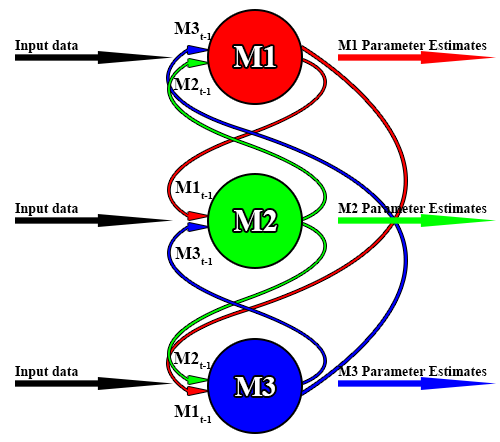
\includegraphics[scale=0.75]{orchestrated_tuning_methodology}
	\caption{Orchestrated tuning of three methods}
	\label{fig:orc_tun_struct}
\end{figure}

%We propose an alternative approach for parameter tuning that uses the fact that we have implementations of multiple methods that attempt to do a similar thing. It features the following iterative process:
%
%1. Initially, each of the methods is trained using the median value of each of its parameters (that is, if the considered values are lambda1= [0.05, 0.1, 1, 10, 20] and lambda2 = [0.1, 0.2, 0.3, 0.4, 0.5], values lambda1=0.1 and lambda2=0.3 will be used) 
%2. Each iteration performs the following for all of the methods:
%- Consider the coefficient vectors of all other methods for the previous iteration, they are averaged to produce the current coefficient vector target
%- Consider combinations of parameter values that are located in the grid next to the previously used set of parameters (in the example from 1. those would be lambda1=[0.1, 1, 10] and lambda2=[0.2, 0.3, 0.4] because the parameters chosen by the previous iteration would be lambda1=0.1 and lambda2=0.3)
%- Fit the method with each of the parameter combinations described above, in this case 9 combinations
%- Consider the coefficient vectors produced by each of the 9 parameter combinations, choose the parameter combination that results in the largest correlation between its coefficient vector and the coefficient vector target (the one we obtained from all other methods)
%- The method's output for the current iteration is the best of the 9 parameter combinations, along with the coefficient vector it produces
%3. Repeat the iterations described in 2. until the movement along the parameter grid is settled (that is, for the latest iteration none of the methods has selected different parameters than the previous iteration)
%4. The parameter values of the last iteration are to be considered optimal for their respective method 
%
%Such a parameter tuning process finds such values for the various methods' parameters that lead to the production of similar coefficient vectors across methods. As explained earlier, the focus is on the predictor coefficients that are estimated in each iteration and not on the prediction error, this is why cross validation is not needed and the parameter tuning process is optimized in terms of computing power. What is more, it uses the fact that we have multiple methods and they perform their parameter tuning cooperatively so as to ensure consensus across methods after the training with arbitrary data.